\documentclass[pdf]{beamer}
\mode<presentation>{}
\usepackage{minted}
\usepackage{tikz}
\usepackage{pgffor} %% gives looping with \foreach
\usepackage[absolute,overlay]{textpos}
\usepackage{lmodern} %% scalable latin characters
\usetikzlibrary{arrows,shapes,backgrounds}
\usepackage{multirow}
\usepackage{listings} %% another package for code related stuff


%% stuff for minted
\definecolor{mintedBg}{rgb}{0.95, 0.95, 0.95}
\definecolor{blockBg}{rgb}{0.6, 0.6, 0.95}
\definecolor{rnaColor}{rgb}{0, 0.6, 0}
\definecolor{cdsColor}{rgb}{0, 0.4, 0.4}
\definecolor{rnaPol}{rgb}{0.8,0,0.8}
\definecolor{ribosomeCol}{rgb}{0.5,0.5,0.1}
\definecolor{protColor}{rgb}{0.6,0,0.6}
%% colours for nucleotides:
\definecolor{dACol}{rgb}{0.5, 0.5, 0}
\definecolor{dCCol}{rgb}{0.8, 0, 0}
\definecolor{dGCol}{rgb}{0, 0.8, 0}
\definecolor{dTCol}{rgb}{0, 0, 0.8}

\definecolor{navy}{rgb}{0, 0, 0.6}
\definecolor{pur}{rgb}{0, 0, 0.6}
\definecolor{pyr}{rgb}{0.6, 0, 0.2}
%% define styles for different codes
\newminted{cpp}{linenos, bgcolor=mintedBg, fontsize=\footnotesize}
%% then use \begin{cppcode}
\newminted{c}{linenos, bgcolor=mintedBg, fontsize=\footnotesize}
\newminted{perl}{linenos, bgcolor=mintedBg, fontsize=\tiny}
\newminted{sh}{linenos, bgcolor=mintedBg, fontsize=\footnotesize,
  language=bash}
\newminted{console}{linenos, bgcolor=mintedBg, fontsize=\tiny}

%% a command to define a subheading
\newcommand\subHeading[1]{
  \par\bigskip {\Large\bfseries#1}\par\smallskip
}

%% I detest indentation in footnotes etc, so try this:
\makeatletter
\renewcommand\@makefntext[1]{\noindent\makebox[0em][r]{\@makefnmark}\tiny#1}
\makeatother
%% the makeatletter and makeatother are required to allow me to
%% to change the macro beginning with an @. (though when I call it
%% I don't use the @ ... 

\setlength\parskip{0.5em}
\setlength\parindent{0ex}

%% to have footnotes without references. This from tex.stackexchange.com
\newcommand\blfootnote[1]{%
  \begingroup  %% this makes it a local redefinition
  \renewcommand\thefootnote{}\footnote{#1}%
  \addtocounter{footnote}{-1}  % this adjusts the footnote counter
  \endgroup
}


\title{Tools for sequence analysis}
\subtitle{running your own}
\author{Martin Jakt}

\begin{document}

\begin{frame}
  \titlepage
\end{frame}

\begin{frame}{Useful tools}
  \begin{itemize}
  \item blast
    \begin{itemize}
    \item creating blast database files
    \item running blast on these
    \end{itemize}
  \item blat : fast database search
  \item clustal : multiple alignment
  \item phylip : old collection of phylogenetic tools
  \item samtools : looking at next generation sequence alignments
  \end{itemize}
  
  blast (detail) and blat covered today.

\end{frame}

\begin{frame}{Installation}
  How to install tools depends on the operating system. Two general options:
  \begin{itemize}
  \item Installation of compiled binaries
    \begin{itemize}
    \item Installation files (Windows), self run archives usually do
      everything fairly automatically.
    \item Install packages from repositories (Linux). Work well when
      available, but often not up to date.
    \item MacOS: for graphical applications usually self-contained
      directory. Not sure for command line utilities, but generally no big
      problem.
    \end{itemize}
  \item Compilation of source code. Generally only for Linux.
  \end{itemize}
\end{frame}

\begin{frame}{Installing from source}
  Well behaved packages usually :
  \begin{enumerate}
  \item ./configure. This checks the system to make sure it has all the
    required dependancies, and creates a suitable Makefile.
  \item make. This runs make on the Makefile which will run the necessary
    commands to compile the program properly (hopefully).
  \item make install. This copies the binaries into suitable directories
    (i.e. ones in the PATH). This usually defaults to \texttt{/usr/local/bin},
    but can be set as an option to the \texttt{./configure} command.
  \end{enumerate}
  
  Installing from source gives you the greatest amount of control over how the
  application will behave, and is generally less work for the developers. For
  bioinformatics tools it usually works, but:\\
  There are many types of problems you can run into.
\end{frame}

\begin{frame}{Geting help}
  Many programs will print usage information if you do one of the following:
  \begin{itemize}
  \item Run the program without any arguments. eg:\\
    \texttt{blastn}
  \item Run the program with the -h, --help or -help switches:\\
    \texttt{blastn -help}\\
    \texttt{samtools --help}\\
    \texttt{samtools view --help}
  \item Use the man program:\\
    \texttt{man samtools}
  \end{itemize}
  
  Sometimes this produces a lot of output: pipe to more or less\footnote{less
    is more} to read it:

  \texttt{samtools view --help | more}
\end{frame}

\begin{frame}[fragile]{Help !}
  \begin{consolecode}
    DL380p:[~]$ samtools --help
    
    Program: samtools (Tools for alignments in the SAM format)
    Version: 1.3.1-36-g613501f (using htslib 1.3.1-52-g0de7fe5)
    
    Usage:   samtools <command> [options]
    
    Commands:
    -- Indexing
    dict           create a sequence dictionary file
    faidx          index/extract FASTA
    index          index alignment
    
    -- Editing
    calmd          recalculate MD/NM tags and '=' bases
    fixmate        fix mate information
    reheader       replace BAM header
    rmdup          remove PCR duplicates
    targetcut      cut fosmid regions (for fosmid pool only)
    addreplacerg   adds or replaces RG tags
    
    -- Viewing
    flags          explain BAM flags
    tview          text alignment viewer
    view           SAM<->BAM<->CRAM conversion
    depad          convert padded BAM to unpadded BAM
    ...
  \end{consolecode}
\end{frame}

\begin{frame}[fragile]{Help !!}
    \begin{consolecode}
      > samtools view --help | more
      Usage: samtools view [options] <in.bam>|<in.sam>|<in.cram> [region ...]

      Options:
      -b       output BAM
      -C       output CRAM (requires -T)
      -1       use fast BAM compression (implies -b)
      -u       uncompressed BAM output (implies -b)
      -h       include header in SAM output
      -H       print SAM header only (no alignments)
      -c       print only the count of matching records
      -o FILE  output file name [stdout]
      -U FILE  output reads not selected by filters to FILE [null]
      -t FILE  FILE listing reference names and lengths (see long help) [null]
      -L FILE  only include reads overlapping this BED FILE [null]
      -r STR   only include reads in read group STR [null]
      -R FILE  only include reads with read group listed in FILE [null]
      -q INT   only include reads with mapping quality >= INT [0]
      -l STR   only include reads in library STR [null]
      -m INT   only include reads with number of CIGAR operations consuming
      query sequence >= INT [0]
      -f INT   only include reads with all bits set in INT set in FLAG [0]
      ...
    \end{consolecode}
    
    learn to read the help and man syntax.
\end{frame}

\begin{frame}{A situation}
  \begin{itemize}
  \item We have short next generation sequences from Monkfish.
  \item We think that it might be lacking in MHC type II genes.\\
    Cod lack these genes and this has some interesting effects on
    immune responses.
  \end{itemize}
  
  What we can do:
  \begin{enumerate}
  \item Make initial assembly
  \item blast MHC (both type I and II) sequences against the assembly
  \item blast the assembly vs MHC sequences\\
    (better to blast against all peptide sequences, but first do quick and
    dirty screen)
  \end{enumerate}
  
  i.e. we do recipocral blast to identify orthologues
  
\end{frame}

\begin{frame}{To run blast}
  \begin{enumerate}
  \item Get MHC type sequences
  \item Create database
  \item Run blast...
  \item Look at the output
  \end{enumerate}

  so lets do that
\end{frame}

\begin{frame}{MHC protein sequences}
  \tiny{
  \begin{tabular}{ ll }
    ENSDARG00000074765  &    major histocompatibility complex class I ZJA \\
    ENSDARG00000092162   &   major histocompatibility complex class I ZAA \\
    ENSDARG00000104293   &   major histocompatibility complex class I ZKA \\
    ENSDARG00000001470    &  major histocompatibility complex class I ZEA \\
    ENSDARG00000079105   &   major histocompatibility complex class II DAB gene \\
    ENSDARG00000056330   &   major histocompatibility complex class II DBB gene \\
    ENSDARG00000036588   &   major histocompatibility complex class I ZBA \\ 
    ENSDARG00000069471  &    major histocompatibility complex class I ZCA \\
    ENSDARG00000088022   &   major histocompatibility complex class I ZFA \\
    ENSDARG00000016056   &   major histocompatibility complex class I LAA \\
    ENSDARG00000096830  &    major histocompatibility complex class I LJA \\
    ENSDARG00000051712   &   major histocompatibility complex class I LFA \\
    ENSDARG00000023203   &   major histocompatibility complex class I LDA \\
    ENSDARG00000096977   &   major histocompatibility complex class I LLA \\
    ENSDARG00000051713   &   major histocompatibility complex class I LGA \\
    ENSDARG00000097766   &   major histocompatibility complex class I LIA \\
    ENSDARG00000092731   &   major histocompatibility complex class I UKA \\
    ENSDARG00000075963  &    major histocompatibility complex class I UBA \\
    ENSDARG00000036628   &   CD74 molecule, major histocompatibility complex,
    class II invariant chain b \\
    ENSDARG00000009087    &  CD74 molecule, major histocompatibility complex, class
    II invariant chain a  \\
    ENSDARG00000090851   &   class II, major histocompatibility complex,
    transactivator  \\
  \end{tabular}
  }
  
  obtained from Ensembl (using raw SQL access).
\end{frame}

\begin{frame}[fragile]{Make db}
  \begin{consolecode}
    makeblastdb
  \end{consolecode}
  
  \begin{itemize}
  \item For the MHC peptide sequences
  \item For the assembly sequences
  \end{itemize}
\end{frame}

\begin{frame}[fragile]{makeblastdb}
    \begin{consolecode}
      lmj:[MHC]> makeblastdb -help | more
      USAGE                                                                                                                                                                 
      makeblastdb [-h] [-help] [-in input_file] [-input_type type]                                                                                                        
      -dbtype molecule_type [-title database_title] [-parse_seqids]                                                                                                     
      [-hash_index] [-mask_data mask_data_files] [-mask_id mask_algo_ids]                                                                                               
      [-mask_desc mask_algo_descriptions] [-gi_mask]
      [-gi_mask_name gi_based_mask_names] [-out database_name]
      [-max_file_sz number_of_bytes] [-logfile File_Name] [-taxid TaxID]
      [-taxid_map TaxIDMapFile] [-version]
      
      DESCRIPTION
      Application to create BLAST databases, version 2.4.0+
      
      REQUIRED ARGUMENTS
      -dbtype <String, `nucl', `prot'>
      Molecule type of target db
      ...
    \end{consolecode}
    
    \tiny{
      \begin{itemize}
      \item \texttt{-in} Specifies the sequence to be converted to a database
      \item \texttt{-input\_type} The format of the sequence data
      \item \texttt{-dbtype} The type of db (i.e. protein or nucleotide)
      \item \texttt{-title} The title of the database (names of the files)
      \end{itemize}

      \verb|[-option]| indicates an optional argument\\
      \verb|[-in input_file]|  you don't need to specify an input file?
    }
\end{frame}

\begin{frame}[fragile]{makeblastdb}
    \begin{consolecode}
      lmj:[MHC]> makeblastdb -help | more
      USAGE                                                                                                                                                                 
      makeblastdb [-h] [-help] [-in input_file] [-input_type type]                                                                                                        
      -dbtype molecule_type [-title database_title] [-parse_seqids]                                                                                                     
      [-hash_index] [-mask_data mask_data_files] [-mask_id mask_algo_ids]                                                                                               
      [-mask_desc mask_algo_descriptions] [-gi_mask]
      [-gi_mask_name gi_based_mask_names] [-out database_name]
      [-max_file_sz number_of_bytes] [-logfile File_Name] [-taxid TaxID]
      [-taxid_map TaxIDMapFile] [-version]
      
      DESCRIPTION
      Application to create BLAST databases, version 2.4.0+
      
      REQUIRED ARGUMENTS
      -dbtype <String, `nucl', `prot'>
      Molecule type of target db
      ...
    \end{consolecode}

    \footnotesize{
      Commands; peptide sequences are in \verb|mhc_peptides.fa|,
      assembled contigs are in \verb|Illumina_assembly.fasta|
    }
    \begin{consolecode}
      > makeblastdb -in mhc_peptides.fa -dbtype prot -title MHC_peptide -out MHC_peptide
      > makeblastdb -in Illumina_assembly.fasta -dbtype nucl -title Il_mf -out Il_mf
    \end{consolecode}
     
\end{frame}

\begin{frame}[fragile]{making the MHC database}
    \begin{consolecode}
      > makeblastdb -in mhc_peptides.fa -dbtype prot -title MHC_peptide -out MHC_peptide
      Building a new DB, current time: 10/20/2016 09:22:27
      New DB name:   /home/lmj/hts2016/assembly/MHC/MHC_peptide
      New DB title:  MHC_peptide
      Sequence type: Protein
      Keep MBits: T
      Maximum file size: 1000000000B
      Adding sequences from FASTA; added 21 sequences in 0.0129869 seconds.

      > ls -lh
      lrwxrwxrwx 1 lmj lmj  164 okt.  20 09:17 Illumina_assembly.fasta
      -rw-rw-r-- 1 lmj lmj 3,9K okt.  20 09:22 MHC_peptide.phr
      -rw-rw-r-- 1 lmj lmj  240 okt.  20 09:22 MHC_peptide.pin
      -rw-rw-r-- 1 lmj lmj 7,7K okt.  20 09:22 MHC_peptide.psq
      -rw-rw-r-- 1 lmj lmj  11K juni  22 11:05 mhc_peptides.fa
    \end{consolecode}
    
    \footnotesize{
      This creates three new files: these files comprise the database.\\
      These files are rather small.
    }
\end{frame}

\begin{frame}[fragile]{Making the assembly database}
  \begin{consolecode}
    > makeblastdb -in Illumina_assembly.fasta -dbtype nucl -title Il_mf -out Il_mf

    Building a new DB, current time: 10/20/2016 09:39:24
    New DB name:   /home/lmj/hts2016/assembly/MHC/Il_mf
    New DB title:  Il_mf
    Sequence type: Nucleotide
    Keep MBits: T
    Maximum file size: 1000000000B
    FASTA-Reader: Ignoring invalid residues at position(s): On line 4: 42
    FASTA-Reader: Ignoring invalid residues at position(s): On line 713: 49
    ...
    FASTA-Reader: Ignoring invalid residues at position(s): On line 13523403: 15
    Adding sequences from FASTA; added 413290 sequences in 33.4144 seconds.
  \end{consolecode}

  \footnotesize Warnings produced due to IUPAC ambiguity codes in assembly.
\end{frame}

\begin{frame}[fragile]{Tidy things up a bit}
  \begin{consolecode}
    lmj:[MHC]> ls -lh
    total 239M
    lrwxrwxrwx 1 lmj lmj  164 okt.  20 09:17 Illumina_assembly.fasta ->
    /home/lmj/hts2016/assembly/Illumina/IlluminaDeNovoAssembly_assembly/IlluminaDeNovoAssembly_d_results/IlluminaDeNovoAssembly_LargeContigs_out_AllStrains.padded.fasta
    -rw-rw-r-- 1 lmj lmj  38M okt.  20 09:39 Il_mf.nhr
    -rw-rw-r-- 1 lmj lmj 4,8M okt.  20 09:39 Il_mf.nin
    -rw-rw-r-- 1 lmj lmj 188M okt.  20 09:39 Il_mf.nsq
    -rw-rw-r-- 1 lmj lmj 3,9K okt.  20 09:22 MHC_peptide.phr
    -rw-rw-r-- 1 lmj lmj  240 okt.  20 09:22 MHC_peptide.pin
    -rw-rw-r-- 1 lmj lmj 7,7K okt.  20 09:22 MHC_peptide.psq
    -rw-rw-r-- 1 lmj lmj  11K juni  22 11:05 mhc_peptides.fa
  \end{consolecode}
  
  \small This is a bit messy. At least move the database files into a seperate
  directory:

  \begin{consolecode}
    > mkdir blastdb
    > mv *.p* blastdb/
    > mv *.n* blastdb/
    > ls -lh blastdb/
    total 230M
    -rw-rw-r-- 1 lmj lmj  38M okt.  20 09:39 Il_mf.nhr
    -rw-rw-r-- 1 lmj lmj 4,8M okt.  20 09:39 Il_mf.nin
    -rw-rw-r-- 1 lmj lmj 188M okt.  20 09:39 Il_mf.nsq
    -rw-rw-r-- 1 lmj lmj 3,9K okt.  20 09:22 MHC_peptide.phr
    -rw-rw-r-- 1 lmj lmj  240 okt.  20 09:22 MHC_peptide.pin
    -rw-rw-r-- 1 lmj lmj 7,7K okt.  20 09:22 MHC_peptide.psq
  \end{consolecode}
\end{frame}

\begin{frame}[fragile]{run blast}
  \begin{itemize}
  \item Protein vs nucleic acid database\\
    \verb|tblastn| (protein query-translated subject)
  \item nucleic acid vs protein database \\
    \verb|blastx| (translated query - protein subject)
  \end{itemize}
\end{frame}

\begin{frame}[fragile]{MHC vs assembly}
  \begin{consolecode}
    > tblastn -help | more
    USAGE
    tblastn [-h] [-help] [-import_search_strategy filename]
    [-export_search_strategy filename] [-task task_name] [-db database_name]
    [-dbsize num_letters] [-gilist filename] [-seqidlist filename]
    [-negative_gilist filename] [-entrez_query entrez_query]
    [-db_soft_mask filtering_algorithm] [-db_hard_mask filtering_algorithm]
    [-subject subject_input_file] [-subject_loc range] [-query input_file]
    [-out output_file] [-evalue evalue] [-word_size int_value]
    [-gapopen open_penalty] [-gapextend extend_penalty]
    [-qcov_hsp_perc float_value] [-max_hsps int_value]
    [-xdrop_ungap float_value] [-xdrop_gap float_value]
    [-xdrop_gap_final float_value] [-searchsp int_value]
    [-sum_stats bool_value] [-db_gencode int_value] [-ungapped]
    [-max_intron_length length] [-seg SEG_options]
    [-soft_masking soft_masking] [-matrix matrix_name]
    [-threshold float_value] [-culling_limit int_value]
    [-best_hit_overhang float_value] [-best_hit_score_edge float_value]
    [-window_size int_value] [-lcase_masking] [-query_loc range]
    [-parse_deflines] [-outfmt format] [-show_gis]
    [-num_descriptions int_value] [-num_alignments int_value]
    [-line_length line_length] [-html] [-max_target_seqs num_sequences]
    [-num_threads int_value] [-remote] [-comp_based_stats compo]
    [-use_sw_tback] [-in_pssm psi_chkpt_file] [-version]

    DESCRIPTION
    Protein Query-Translated Subject BLAST 2.4.0+
    ...
  \end{consolecode}
  
  ouch, too many options... 
\end{frame}

\begin{frame}[fragile]{tblastn options}
  \small{
  Looking through the options, what do we have, what do we need, and what can
  we guess the meaning of?
  \begin{itemize}
    \item \verb|[-db database_name]|
    \item \verb|[-query input_file]|
    \item \verb|[-out output_file]|
    \item \verb|[-evalue evalue]|
    \item \verb|[-word_size int_value]|
    \item \verb|[-gapopen open_penalty]|
    \item \verb|[-gapextend extend_penalty]|
    \item \verb|[-max_hsps]|
    \item \verb|[-matrix matrix_name]|
    \item \verb|[-outfmt format]|
  \end{itemize}
  }
\end{frame}

\begin{frame}[fragile]{tblastn command}
  So lets build a minimal command:
  \pause

  \verb|tblastn| \pause \verb|-db blastdb/IL_mf| \pause
  \verb|-query mhc_peptides.fa| \pause \verb|-out mhc_ass.out|

  \pause
  \begin{consolecode}
> more mch_ass.out
BLASTN 2.4.0+


Reference: Stephen F. Altschul, Thomas L. Madden, Alejandro A.
Schaffer, Jinghui Zhang, Zheng Zhang, Webb Miller, and David J.
Lipman (1997), ``Gapped BLAST and PSI-BLAST: a new generation of
protein database search programs'', Nucleic Acids Res. 25:3389-3402.



Database: Il_mf 413,290 sequences; 774,336,139 total letters
    
Query= ENSDARP00000135947
Length=407
                                                                      Score  E
Sequences producing significant alignments:                          (Bits)  Value

IlluminaDeNovoAssembly_c207389                                        102    6e-22
IlluminaDeNovoAssembly_rep_c424064                                    69.3   2e-12
IlluminaDeNovoAssembly_rep_c326236                                    71.2   1e-11
IlluminaDeNovoAssembly_rep_c424063                                    70.1   2e-11
...
  \end{consolecode}

\end{frame}

\begin{frame}[fragile]{tblastn output ...}
  \begin{consolecode}
...
IlluminaDeNovoAssembly_rep_c311894                                  33.1  8.3  
IlluminaDeNovoAssembly_rep_c405314                                  32.3  9.8  

> IlluminaDeNovoAssembly_c207389
Length=1802

 Score = 102 bits (253),  Expect = 6e-22, Method: Compositional matrix adjust.
 Identities = 51/105 (49%), Positives = 69/105 (66%), Gaps = 3/105 (3%)
 Frame = +3

Query  12    YLCLFHVIMSSFRAEKHSLYFIYTGLSRPVDLPGIYEFSAMGLLDDRQIDSYNSEEQRNI  71
             +L  F  + SS   E+HSL + YT LS+ V+LPGI+ F+AMGLLD R ID Y+S  +  +
Sbjct  987   HLSAFLFVWSS---ERHSLTYTYTALSKDVNLPGIHPFTAMGLLDKRMIDYYDSVTEEKV  1157

Query  72    PKQQWMKEKMQEDYWENRTQSRKEKQLWFYDNVHLLIDRNRQSTS  116
             PKQ WM+E++  DYW   T+SRK K  WF  N+ +L  R RQ+ S
Sbjct  1158  PKQTWMEERLDADYWLKGTKSRKSKNQWFRVNLDILKKRMRQNDS  1292


 Score = 41.6 bits (96),  Expect = 0.018, Method: Compositional matrix adjust.
 Identities = 18/36 (50%), Positives = 22/36 (61%), Gaps = 1/36 (3%)
 Frame = +3

Query  119   HVLQWRHGCEVEKQGNEH-SFNKSIDEYGYDGEDFL  153
             HVLQWRHGC  +   +   +F   +D Y YDG DFL
Sbjct  1692  HVLQWRHGCVADMNPDGSVTFVSGMDMYSYDGNDFL  1799
...

Query= ENSDARP00000118368
...
  \end{consolecode}
\end{frame}

\begin{frame}[fragile]{blast output format}
  \begin{consolecode}
    > tblastn -help | less
    ...
     *** Formatting options
     -outfmt <String>
     alignment view options:
       0 = Pairwise,
       1 = Query-anchored showing identities,
       2 = Query-anchored no identities,
       3 = Flat query-anchored showing identities,
       4 = Flat query-anchored no identities,
       5 = BLAST XML,
       6 = Tabular,
       7 = Tabular with comment lines,
       8 = Seqalign (Text ASN.1),
       9 = Seqalign (Binary ASN.1),
       10 = Comma-separated values,
       11 = BLAST archive (ASN.1),
       12 = Seqalign (JSON),
       13 = Multiple-file BLAST JSON,
       14 = Multiple-file BLAST XML2,
       15 = Single-file BLAST JSON,
       16 = Single-file BLAST XML2
  \end{consolecode}
  
  \footnotesize Note that options 6, 7, and 10 can be customised to include
  additional columns.
  
  \footnotesize Tabular options are often useful for summarising alignments.
\end{frame}

\begin{frame}[fragile]{tblastn tabular output}
  \begin{consolecode}
> tblastn -db blastdb/Il_mf -query mhc_peptides.fa -out mch_ass.tbl -outfmt 6
> more mch_ass.tbl
ENSDARP0135947      Ill_c207389  48.571  105  51   1    12    116   987    1292    5.70e-22  102
ENSDARP0135947      Ill_c207389  50.000  36   17   1    119   153   1692   179     0.018     41.6
ENSDARP0135947      Ill_c424064  36.449  107  62   2    116   219   516    205     1.77e-12  69.3
ENSDARP0135947      Ill_c326236  37.736  106  60   2    116   218   592    284     1.04e-11  71.2
...
  \end{consolecode}
nice tabular format; can easily be parsed by other programs, eg. import into
R, use \texttt{tapply} to split by protein, etc..
\end{frame}

\begin{frame}[fragile]{blastx command}
  \begin{consolecode}
    > blastx -help
  \end{consolecode}
  Looks very similar to the help for \verb|tblastn|. So we can make a very
  similar command:

  \begin{consolecode}
    > blastx -db blastdb/MHC_peptide -query Illumina_assembly.fasta -out ass_mhc.out
  \end{consolecode}
  
  but that will run more than 400,000 blast queries; which will take quite a
  long time. Maybe around a week. We don't actually have to run all of
  these...
  
\end{frame}

\begin{frame}[fragile]{blat the fast aligner}
  \begin{consolecode}
DL380p:[gadMor2]$ blat -h
-h is not a valid option
DL380p:[gadMor2]$ blat -help
-help is not a valid option
DL380p:[gadMor2]$ blat
blat - Standalone BLAT v. 35 fast sequence search command line tool
usage:
   blat database query [-ooc=11.ooc] output.psl
where:
   database and query are each either a .fa , .nib or .2bit file,
   or a list these files one file name per line.
   -ooc=11.ooc tells the program to load over-occurring 11-mers from
               and external file.  This will increase the speed
               by a factor of 40 in many cases, but is not required
   output.psl is where to put the output.
   Subranges of nib and .2bit files may specified using the syntax:
      /path/file.nib:seqid:start-end
   or
      /path/file.2bit:seqid:start-end
   or
      /path/file.nib:start-end
....
  \end{consolecode}
\end{frame}

\begin{frame}[fragile]{blat the fast mapper}
  Database is our assembly, the query is a temporary file with some partial
  sequences from the assembly.

  Then.. 
  \begin{consolecode}
> blat -makeOoc=11.ooc -ooc=11.ooc -t=dna -q=dna Illumina_assembly.fasta tmp.fa tmp_ass.psl
Loading Illumina_assembly.fasta
Counting Illumina_assembly.fasta
Writing 11.ooc
>
> blat -ooc=11.ooc -t=dna -q=dna Illumina_assembly.fasta tmp.fa tmp_ass.psl
Loaded 774336139 letters in 413290 sequences
Searched 2660 bases in 3 sequences
>
> pslPretty tmp_ass.psl Illumina_assembly.fasta tmp.fa pretty.out
  \end{consolecode}
\end{frame}

\begin{frame}[fragile]{blat output}
  \begin{figure}[ht]
    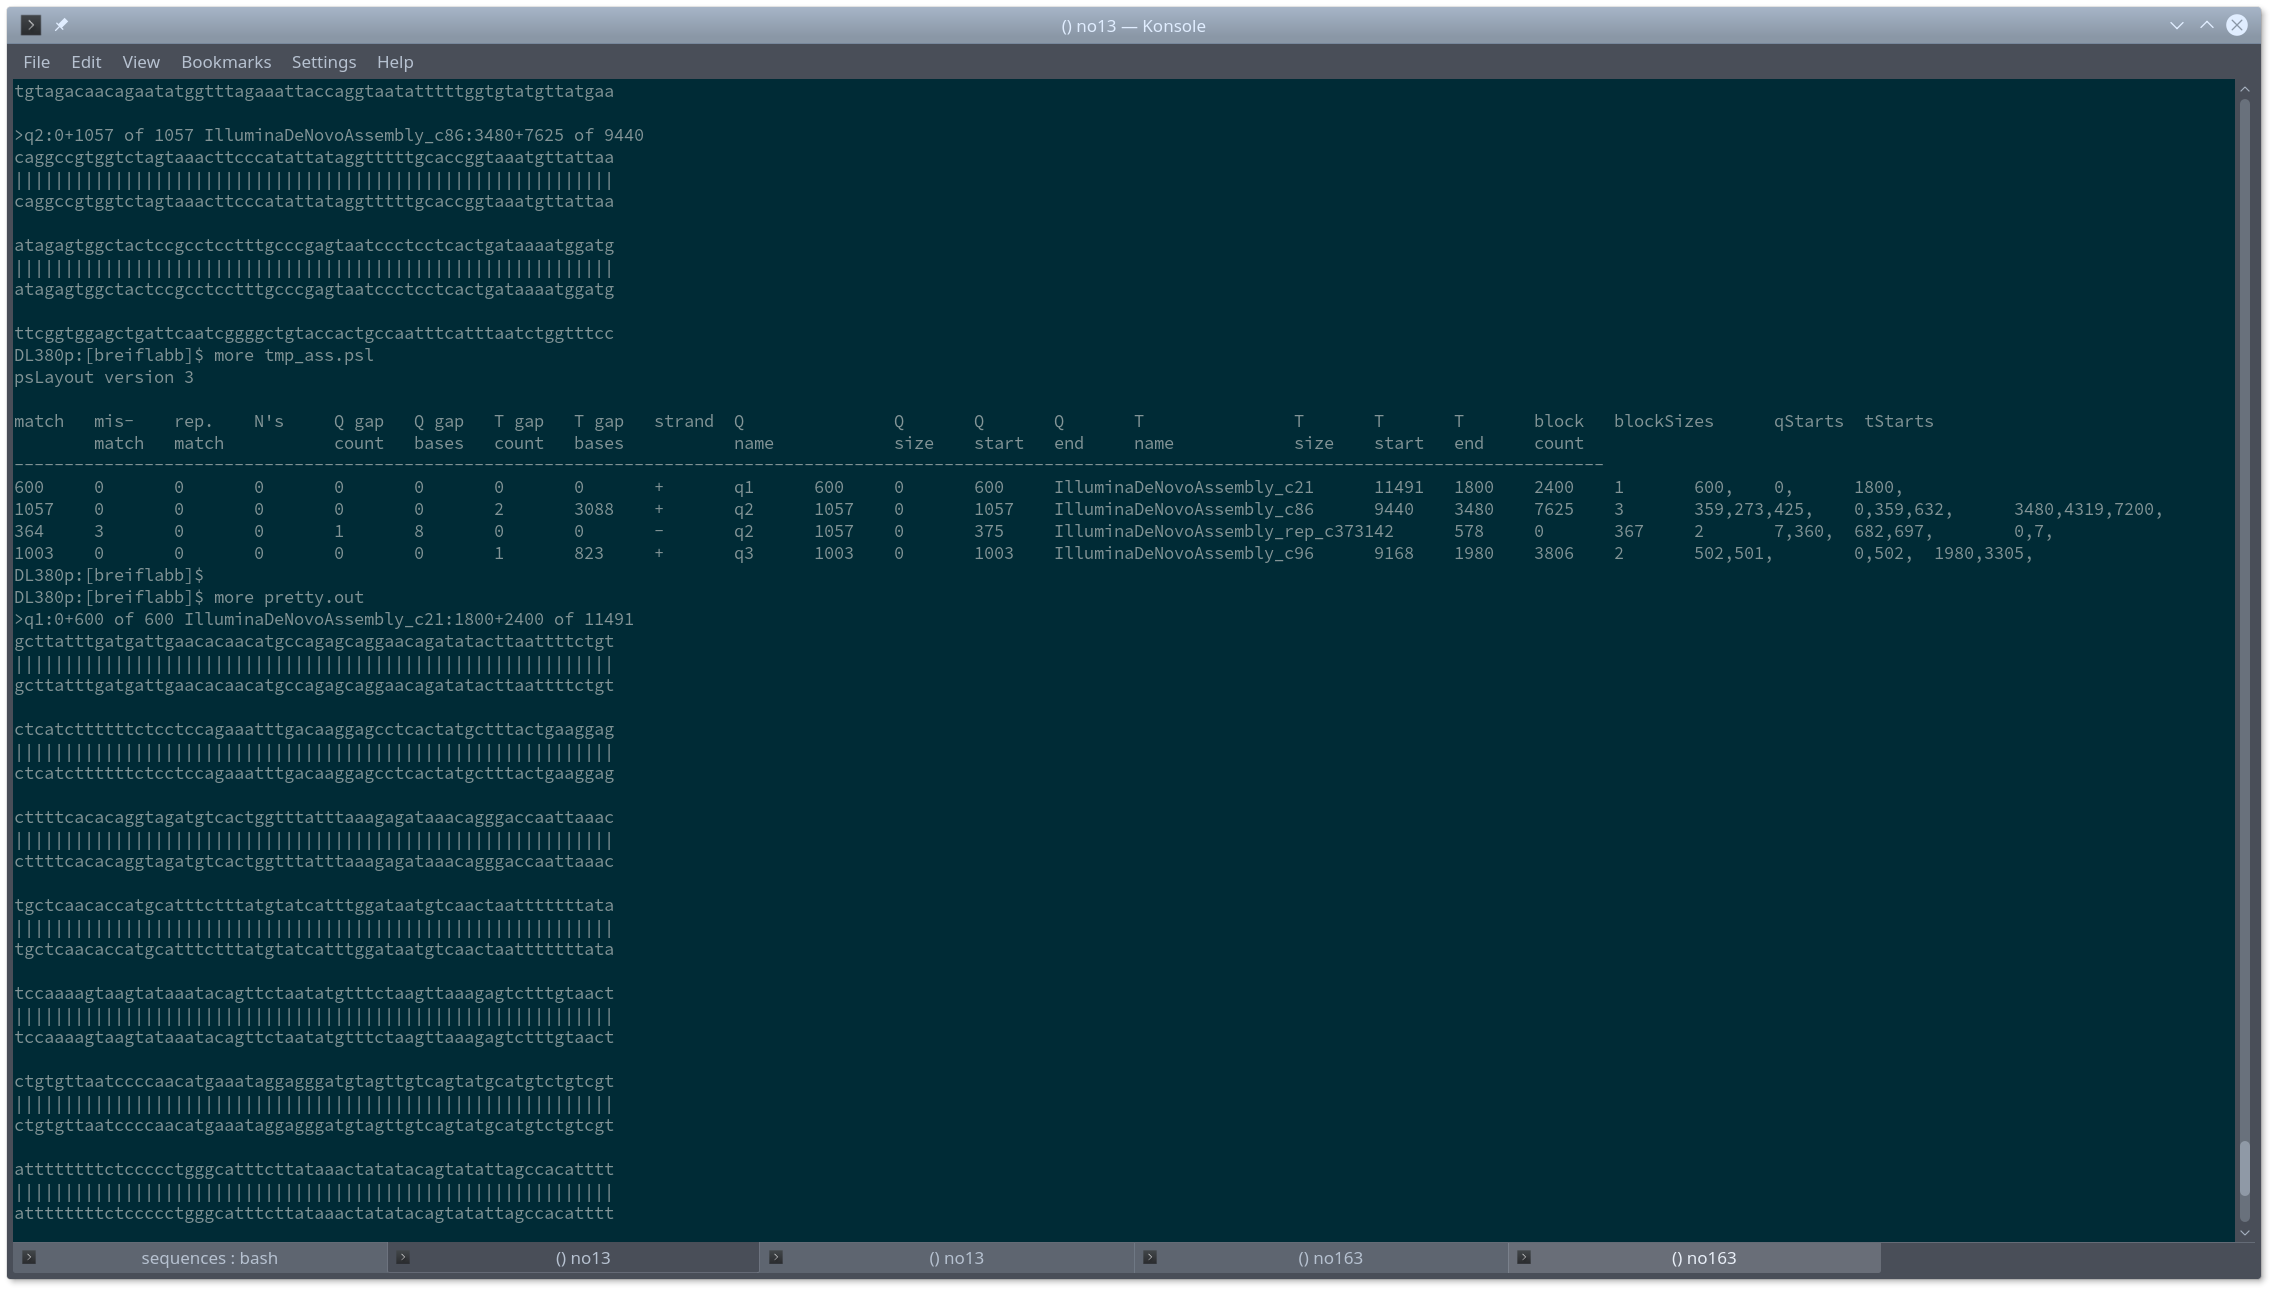
\includegraphics[width=\textwidth]{images/blat_output}
  \end{figure}
  
\end{frame}

\begin{frame}{Exam question?}
  \begin{itemize}
  \item I don't expect you to be able to remember how to run a specific
    program.
  \item I \emph{do} want you to be able to read the help notes and understand
    them reasonably well.
  \item Question in exam may be: given a section of the man page, and the
    names of some files put together a command line that performs a specified
    task.
  \end{itemize}
\end{frame}

\end{document}
